\newpage
\subsection{Caso d'uso UC11 - Registrazione API}
\label{UC11}
\begin{figure}[ht]
	\centering
	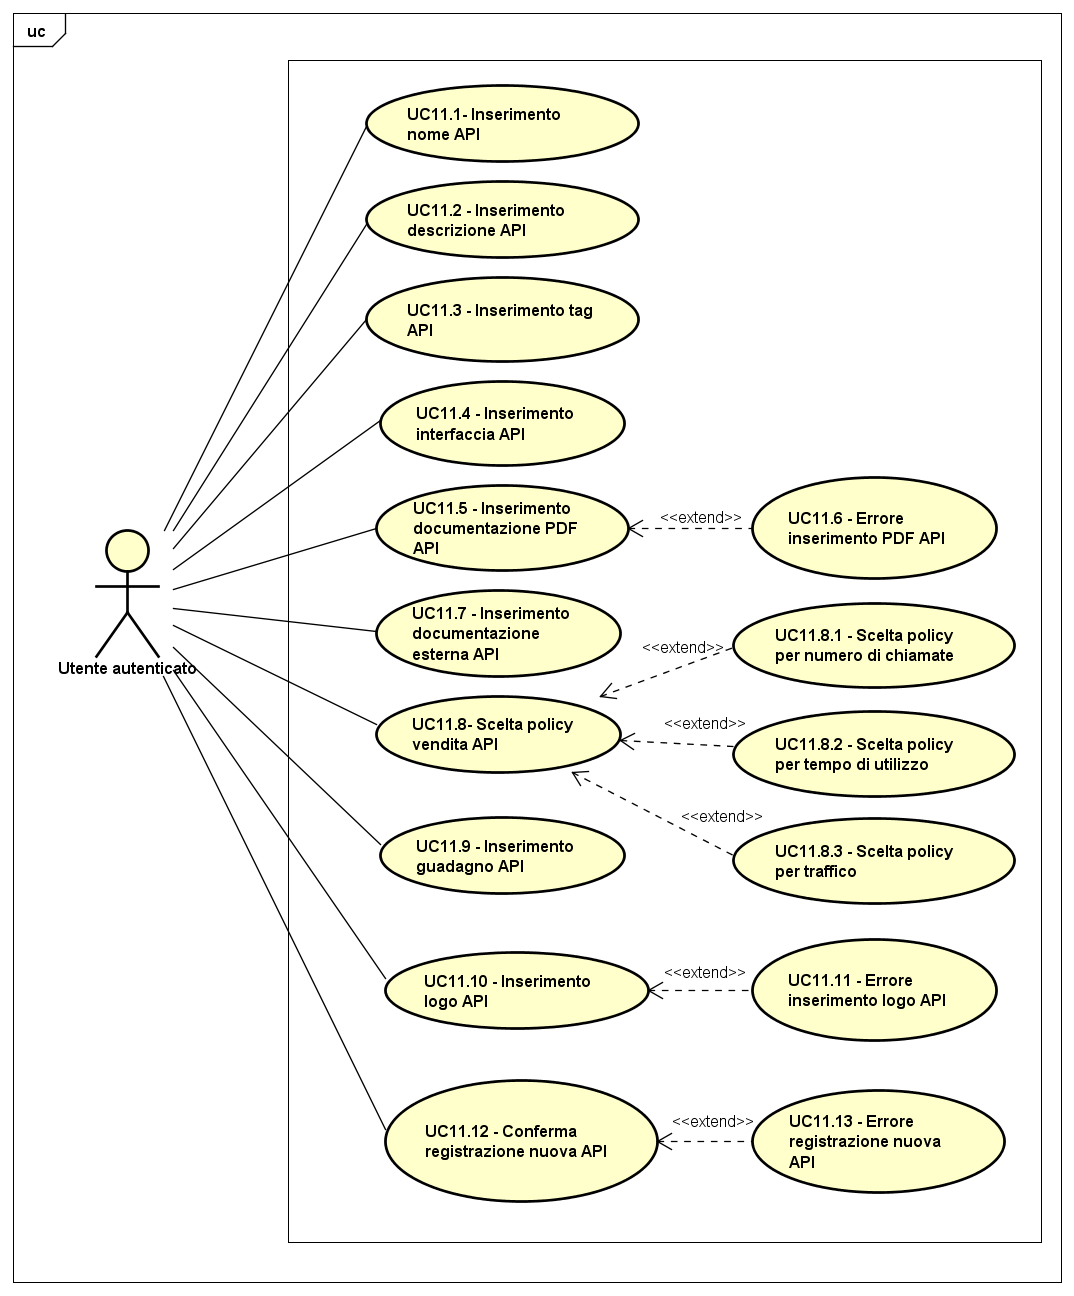
\includegraphics[scale=0.45]{UML/UC11.png}
	\caption{UC10: Registrazione API}
\end{figure}

\begin{longtable}{ l | p{11cm}}
	\hline
	\rowcolor{Gray}
	\multicolumn{2}{c}{UC11 - Visualizzazione API registrate}\\
	\hline
	
	 \textbf{Attori} & Utente autenticato  \\
	\textbf{Descrizione} & L'attore può \\
	\textbf{Pre-Condizioni} & L'attore \\
	\textbf{Post-Condizioni} & L'attore \\
	\textbf{Scenario Principale} & 
	\begin{enumerate*}[label=(\arabic*.),itemjoin={\newline}]
		\item L'attore visualizza
	\end{enumerate*}\\
\end{longtable}


\subsubsection{Caso d'uso UC11.1: Registrazione}
\label{UC11_1}

\begin{minipage}{\linewidth}
	\begin{tabular}{ l | p{11cm}}
		\hline
		\rowcolor{Gray}
		\multicolumn{2}{c}{UC11.1 - Registrazione} \\
		\hline
		\textbf{Attori} & Utente autenticato \\
		\textbf{Descrizione} & L'attore \\
		\textbf{Pre-Condizioni} & L'attore\\
		\textbf{Post-Condizioni} & L'attore\\
		\textbf{Scenario Principale} & 
		\begin{enumerate*}[label=(\arabic*.),itemjoin={\newline}]
			\item L'attore
		\end{enumerate*}\\
	\end{tabular}
\end{minipage}
